%%%%%%%%%%%%%%%%%%%%%%%%%%%%%%%%%%%%%%%%%%%%%%%%%%%%%%%%%%%%%%%%%%%%%%
%
% レポートテンプレート
%
% updated 22 Oct, 2018
% last updated 02 Apr, 2021
%
% (c) Tohru TAKADA@UEC
% 各自のレポートに合わせて変更して使ってください.上記の行は残して使うこと.
% 2次配布可です.ご利用は計画的に.
%
%%%%%%%%%%%%%%%%%%%%%%%%%%%%%%%%%%%%%%%%%%%%%%%%%%%%%%%%%%%%%%%%%%%%%%
\documentclass[a4paper,10pt]{jarticle}
\usepackage[dvipdfmx]{graphicx}
\usepackage{amsmath}
\usepackage{latexsym}
\usepackage{multirow}
\usepackage{url}
\setlength{\textwidth}{165mm} %165mm-marginparwidth
\setlength{\marginparwidth}{40mm}
\setlength{\textheight}{225mm}
\setlength{\topmargin}{-5mm}
\setlength{\oddsidemargin}{-3.5mm}

\def\vector#1{\mbox{\boldmath $#1$}}
\newcommand{\AmSLaTeX}{%
 $\mathcal A$\lower.4ex\hbox{$\!\mathcal M\!$}$\mathcal S$-\LaTeX}
\newcommand{\PS}{{\scshape Post\-Script}}
\def\BibTeX{{\rmfamily B\kern-.05em{\scshape i\kern-.025em b}\kern-.08em
 T\kern-.1667em\lower.7ex\hbox{E}\kern-.125em X}}
\newcommand{\pderiv}[2]{{\partial#1\over\partial#2}}
\newcommand{\deriv}[2]{{{\rm d}#1\over{\rm d}#2}}
\newcommand{\dderiv}[2]{{{\rm d}^2#1\over{\rm d}#2^2}}
\newcommand{\DeLta}{{\mit\Delta}}
\renewcommand{\d}{{\rm d}}
\def\wcaption#1{\caption[]{\parbox[t]{100mm}{#1}}}
\def\rm#1{\mathrm{#1}}
\def\tempC{^\circ \rm{C}}

\makeatletter
%\def\section{\@startsection {section}{1}{\z@}{-3.5ex plus -1ex minus % -.2ex}{2.3ex plus .2ex}{\Large\bf}}
\def\section{\@startsection {section}{1}{\z@}{-3.5ex plus -1ex minus
-.2ex}{2.3ex plus .2ex}{\normalsize\bf}}
\makeatother

\makeatletter
\def\subsection{\@startsection {subsection}{1}{\z@}{-3.5ex plus -1ex minus
-.2ex}{2.3ex plus .2ex}{\normalsize\bf}}
\makeatother

\makeatletter
\def\@seccntformat#1{\@ifundefined{#1@cntformat}%
   {\csname the#1\endcsname\quad}%      default
   {\csname #1@cntformat\endcsname}%    enable individual control
}
\makeatother

%%%%%%%%%%%%%%%%%%%%%%%%%%%%%%%%%%%%%%%%%%%%%%%%%%%%%%%%%%%%%%%%%%%%%%
\begin{document}

%
%% 通常は指定の表紙を付けて印刷して提出していますが,電子データをアップロードする際は
%% 表紙は付けなくても結構です.冒頭にタイトル,所属,学籍番号,氏名と記載日
%% 修正版を提出する際は更新日を書いてください
%
\begin{center}
{\Large{\bf レポートのためのテンプレート}} \\
{\bf 電気通信大学 O類XXプログラム\\
YYXXNNN 電通太郎} \\
{\bf 20YY年O月O日作成} \\
{\bf 20YY年X月X日更新}
\end{center}
%%%%%%%%%%%%%%%%%%%%%%%%%%%%%%%%%%%%%%%%%%%%%%%%%%%%%%%%%%%%%%%%%%%%%%
\section{目的}

 実験の目的は,常にその課題で最終的に求める物理量について,「ooを求める.」といった
書き方をすると良いでしょう.基礎科学実験Aでは「重力加速度の測定」では「重力加速度を
4桁の精度で求める」ことが目的ですし,音の共鳴では「気体や固体中の波の速さ(音速)」を
求めること,「液体の比熱」では「水ならびにアルコールの比熱を加熱法と冷却法によって求める」
ことが目的です.

しかし,目的(続く節でも同様ですが)のセクションにこれだけ(骨格部分のみ)を書いただけでは,
貴方の文章を読んだ読者はこのレポートが無味乾燥でつまらないと思うことでしょう.
ですので,骨格部分に不必要に冗長的にならない程度に枝葉を付けていくことが必要です.
例えば,目的とする量はいったいどのようなものなのか,私たちの世界ではどういった役に
なっているのか,それを調べるとどのようなことが情報として得られるのか,こういったことを
調べて付加えると良いでしょう.

\vspace{3mm}
レポートは,このテンプレートが示すように「セクション構成」にします.各セクションはセクション番号と
セクション見出しを付け「ゴシック体」にして表します.本文は明朝体にしておきます.セクション見出しと
本文は同じフォントサイズを用いるので構いません.少なくとも本文に対してあまりにも大きい
フォントサイズにはしない方が無難です.このテンプレートのソースを見れば,\LaTeX についての
基本的な文法(数式を書くときや図の挿入方法,表の作成方法,参考文献の作り方等々)に
ついてどのように書けばどうなるのかが分かるはずです.テンプレートには出来上がりの
PDFもつけてありますので,よく見比べてください.テンプレートを使うときは必ず別名で
保存してから修正をすることを薦めます.

%%%%%%%%%%%%%%%%%%%%%%%%%%%%%%%%%%%%%%%%%%%%%%%%%%%%%%%%%%%%%%%%%%%%%%
\section{原理}
実験の原理では目的に掲げた求めるべき物理量をどのような物理法則に基づいて求めるのかに
ついて数式を用いて解説します.皆さんが行う測定は,どのような数学的なモデルに
従って分布するのか,この原理のセクションで全て説明がされており,この意味ではどのような
結果を得るのかすでに判明しています.

例えば重力加速度では振子の等時性の式に対して半径が $r$ の剛体球を用いること,および
振子の振れ角が有限の $\theta$ という大きさであることの補正を取り入れた次式が用いられます.
%
\begin{equation}
T=2\pi \sqrt{\frac{h}{g}\left (1+\frac{2r^2}{5h^2}\right )} \times \left (1+\frac{\theta^2}{16}\right )
\label{grav_eq}
\end{equation}

実験の原理では上式で原理を終えるのは良い方法ではありません.なぜなら,あなたが
求めるべき量は重力加速ですから,式(\ref{grav_eq})を $g$ について解いた
ものを載せるのが良い方法です.
%
\begin{equation}
g=\frac{4\pi^2 h}{T^2}\times \left (1+\frac{2r^2}{5h^2} +\frac{\theta^2}{8}\right )
\label{grav2_eq}
\end{equation}

一行独立に書いている式には必ず式番号を割り振ってください.式のインデントの付け方は
分野によって幾つか流儀があるようです.物理では式を中央寄せ,数式番号は右寄せに
して行をそろえるのが一般的です.

\vspace{3mm}
\TeX では数式にはラベル(\verb|\label{<label>}|)を付けておき,後で参照(\verb|\ref{<label>}|)すると
式番号を自動的に引用します(後で途中に式を追加してもいちいち付け直す必要はありません).
ただし,引用は一度のコンパイルでは解決できない場合があります(??のように式番号が未定に
なります.メッセージを読むと警告が表示されているはずです).このようなときは
もう一度コンパイルをしてください.また,式をコピペしているときに起こりがちですが,ラベルは重複して
用いることはできません.ペーストした際はラベルを書き換えることを忘れないでください.

数式を書くのは \TeX に慣れるまでは存外面倒なものです.各課題について代表的な数式を
ここで掲載しておきましょう.どのように数式コマンドを書けばよいかの参考にしてください.

%
\subsection{重力加速度の測定}
不確かさを求める式は次のようになります.
\begin{eqnarray}
\overline{g}=\cfrac{\cfrac{g_1}{(\Delta g_1)^2}+\cfrac{g_2}{(\Delta g_2)^2}+\cdots+\cfrac{g_n}{(\Delta g_n)^2}}{\cfrac{1}{(\Delta g_1)^2}+\cfrac{1}{(\Delta g_2)^2}+\cdots+\cfrac{1}{(\Delta g_n)^2}} \\
\label{eq1}
\Delta g = \cfrac{1}{\sqrt{\cfrac{1}{(\Delta g_1)^2}+\cfrac{1}{(\Delta g_2)^2}+\cdots+\cfrac{1}{(\Delta g_n)^2}}}
\label{eq2}
\end{eqnarray}

%
\subsection{音の共鳴}
固体中の波の速さ $v_m$ に対する合成標準不確かさを求める式.
\begin{equation}
\frac{\Delta v_m}{v_m}=\sqrt{\left (\frac{\Delta L_g}{L_g}\right )^2+\left (\frac{\Delta l_m}{l_m}\right )^2+\left (\frac{\Delta v_g}{v_g}\right )^2}
\label{eq3}
\end{equation}

\subsection{液体の比熱}
加熱法による液体試料の温度上昇と時間の関係を表す式.
\begin{equation}
\frac{\Delta T}{\Delta t}=\frac{Ri^2}{MC+mc}
\label{eq4}
\end{equation}

\subsection{2次元の等電位線}
中央に導体がある等電位線の理論式の作図に関する式.
\begin{equation}
x=\pm \sqrt{\frac{y(-y^2+cy+R^2)}{y-c}}
\label{eq5}
\end{equation}

\subsection{電気回路}
抵抗,コイル,コンデンサの直列回路による過渡応答の原理式.
\begin{equation}
\dderiv{I(t)}{t}+2\gamma \deriv{I(t)}{t}+\omega_0^2I(t)=0
\label{eq6}
\end{equation}

ここで用いている\verb|\ddereiv|や\verb|\deriv|はこのファイルの冒頭に定義してあるもので,通常の
\TeX のコマンドではないことに注意が必要です.

\subsection{ヤング率}
たわみによるヤング率を求める式.
\begin{equation}
E=\frac{g}{2}\frac{l^3 d}{a^3 br}\frac{m}{S-S_0}
\label{eq7}
\end{equation}

\subsection{粘性率}
ポアズイユの法則を表す式.
\begin{equation}
p_1-p_2=\left (\rho g\cos\theta -\frac{2\gamma}{al}\right )l
\label{eq8}
\end{equation}

\subsection{光のスペクトル}
Na線の D$_1$線とD$_2$線の波長.

 D$_1$線:589.592 nm \\
 
 ${\rm D_2}$線:588.995 $\rm{nm}$

 \vspace{2mm}
 上記は同じ表示になるものを異なる方法で表記しています.ただし\verb|\rm|のコマンドは
 このファイルの冒頭で再定義しており,\TeX の本来のコマンドとは異なる挙動をしています.
 
\subsection{エアトラックによる力学実験}
滑走体のエアトラック上の運動方程式を減速の平均の加速度 $\overline{a}$ と平均速度 $\overline{v}$ で記述した式.
\begin{equation}
\frac{\overline{a}}{g}=\mu \cos\theta +\left (\frac{\lambda}{mg}\right )\overline{v}+\left (\frac{\kappa}{mg}\right )\overline{v}^2\mp\sin\theta
\label{eq9}
\end{equation}

\subsection{放射線の計測}
放射性同位元素セシウム137のベータ崩壊様式.

\begin{equation}
^{137}_{\hspace{1.2mm}55}\rm{Cs} \rightarrow ^{137}_{\hspace{1.2mm}56}\rm{Ba} + \rm{e}^{-} +\overline{\nu}_{\rm{e}}
\label{beta-colps}
\end{equation}

%%%%%%%%%%%%%%%%%%%%%%%%%%%%%%%%%%%%%%%%%%%%%%%%%%%%%%%%%%%%%%%%%%%%%%
\section{方法}
 原理で目的とする物理量を求めるために利用する法則を数式で説明をしました.
実験はテストの問題と異なり,それに基づいて測定器や実験装置を用いて測定値を得ることに
なります.このセクションに続く「実験結果」のセクションでデータを羅列しても,
一体どのようにそれを
測ったのかを説明しなければ読者は理解することはできません.このセクション「実験方法」で
主に書く内容は,
測定装置としてどのようなものを用いたのか,また測定手法はどのようなものであったのかを
説明をになります.ここで注意して欲しいことは,
「測定手法」を説明する際に,手順を逐一全て(マニュアルのように)書く必要はないということです.
\footnote{
実験テキストは,これを読んだ皆さんが上手に測定をできるように細かい手順を
書いていますが,皆さんはそれを参照して測定を行い,その結果をレポートに
まとめているのですから,オウム返しに同じことを書く必要はないのです.
}
実験方法のセクションに書く内容は時と場合によって異なるので唯一これを書いておけば
大丈夫といった処方箋はありません.ただ実験授業で与える課題の範疇では各範囲は
それほど振れ幅はないく,良い訓練の機会となります.このセクションで書く内容の
ポイントとしては次のような事柄を押さえるつもりで記載すると良いでしょう.

%
\begin{itemize}
\setlength{\itemsep}{-2mm}
 \item 測定上特に注意をした点(注意をしなければならなかった点)
 \item 測定装置で特に説明をしなければ何故,どのように測定値を取得したのか
 	  読者にわからない点
 \item 実験結果を再現するために必要な特別な手順や測定方法など
 \item 測定データを処理する際に利用したソフトウェアで特に記載が必要なもの
\end{itemize}

記載内容全般に渡って言えることですが,理工系の実験レポートの読者は任意の他者ではなく,
同程度の知識を有していることを前提で,このため同じ分野の人間にとって常識となっていることや,
暗黙の了解となっていることは説明することはありません.散見される例として,例えば電圧を
測ることに対し,実験方法で次のような箇条書きをしたらどうでしょうか?
%
\begin{enumerate}
\setlength{\itemsep}{-2mm}
 \item 電圧はディジタルマルチメーターを用いて測った
 \item まずディジタルマルチメーターの電源をONにした
 \item 次にメーターのプローブを電源端子に接続し$\cdots$
\end{enumerate}

電圧を測る手段はそう多くはなく,およそまず「ディジタルマルチメーター」を想像するでしょう.
また電気製品は電源を入れなけば動作しないことは万人が知っていることですし,
プローブの類を端子に接触させなければ測れないのも当然のことでしょう.

実験方法のセクションでは,以上のようにまず実験装置の概略図を載せます.そして,本当に
説明が必要なことだけを説明しするので十分なのです.装置の図は
本当に簡単なものでよく(凝ったイラストやカラーを用いる必要はありません.直線,四角,円で
書いたようなもので十部です),ただし説明したい箇所を漏らさずに記載します.なお,作図を
する場合に \TeX では EPS という形式のファイルを扱う方が仕上がりがきれいに
出来ます.INKSCAPE 等フリーのツールもありますので活用してください.

\vspace{3mm}
一例として「液体の比熱」について詳しい説明をしましょう.この実験は液体の比熱を
加熱法と冷却法で求めます.液体試料は「恒温槽」に格納されます.この恒温槽は
水道水を常に流し込み一定の温度に保つという大変シンプルなものですが,この
「流水の温度」が測定最中に変化しないかは大変重要な問題です.このため,
実験中は流水の温度(環境温度) $T_\rm{A}$ を何回か測定をします.

液体試料は均一温度になるよう「常に攪拌」を行う必要があります.攪拌のやり方が
乱暴であると液体試料は容器からこぼれてしまいます.いずれにしても加熱や冷却で
質量は変化する可能性が高く,このため実験では「液体試料の質量」を測定の
前後で必ず2回測ります.

加熱は 5$\sim$6 $\rm{\Omega}$ のマンガニン線をコイル状にし,そこに電流を
流してジュール熱を発生させて熱源とします.マンガニン線が空気中に露出すると
焼損をする可能性が高く,往々にして(慎重に攪拌したとしても)マンガニン線が焦げて
しまったという事故が起こります.この際に重要なのはどの時点でそれが発生したかに
なります(実験開始直後であれば測定を中止してやり直した方が早く,2/3程度
データが取得出来ていればそのまま続けても良い可能性があります).そこで,
測定最中「電流値」に変動がないか度々チェックしていることが重要です.また,
焦げていた場合は事後に「抵抗値を再度測定」して大きな変化がないか
確認する必要もあります.

以上が液体の比熱(加熱法)のあらましです.では,この実験について「実験方法」を
どのように書けばよいでしょうか?上で「」で囲った部分は重要な(私が読者に説明したいと
考えた)ポイントです.そこで,次のような文章と装置の図を書くことにしましょう.

\vspace{3mm}
\hrulefill

この実験では以下のような装置(図\ref{apara}参照)を用いて測定を行った。
液体試料を入れた熱量計を恒温槽(流水で内部を一定に保っている)に設置し(
恒温槽の底面と熱量計はスペーサーで断熱されている),熱量計には攪拌棒などが
入った状態で加熱用の蓋または冷却用の蓋で上部がふさがれる.
%
\begin{figure}[ht]
\begin{center}
 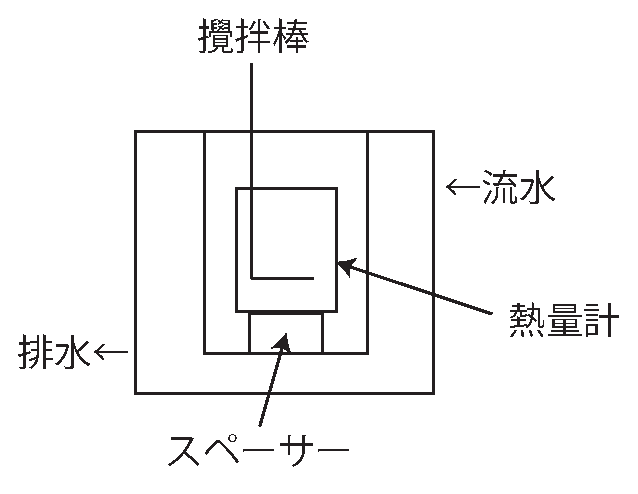
\includegraphics[scale=0.6]{aparatus2.eps}
 \caption{実験装置の概略図}
 %\ecaption{Options of documentclass.}
\label[apara]
\end{center}
\end{figure}

流水の温度は「環境温度 $T_\rm{A}$」として測定最中に変化がないか幾度か
記録している.加熱実験では電源からアナログ電流計を介して加熱用蓋まで配線した.
測定中には電流値の変動がないか,やはり数度確認して記録した.

攪拌棒による液体試料の攪拌は,早すぎると液体試料をこぼす原因となり,逆に
遅すぎても十分攪拌ができないことから特に留意して測定を行った.具体的には
およそo秒に1回程度,上下のストロークをx cm程度取って行っている.攪拌以外にも
液体試料の質量の変化は不可避であるため,測定の前後で試料の質量を
測定しており,この結果については考察で吟味している.

\hrulefill

%%%%%%%%%%%%%%%%%%%%%%%%%%%%%%%%%%%%%%%%%%%%%%%%%%%%%%%%%%%%%%%%%%%%%%
\section{実験結果}

 実験結果のセクションでは得られた測定値を元にして目的のセクションで掲げた物理量を
計算し,(存在する場合は)比較できる文献値等と一緒に最後に表にしてまとめます.もちろん,
不確かさや精度を吟味できる場合,同様のこのセクションで計算を行って求めた値と合わせて示します.

データをまとめる際は必ず表にしてまとめてください.またはデータを
グラフにプロットして表示することは良いアイディアで,多くの場合傾向が大変分かりやすくなります.
表やグラフをどのように書くのかについてはeラーニングの課題として与えています.よく習熟して
ください.表のサンプルは次の表\ref{tab1}のようなものです.
%
\begin{table}[ht]
\begin{center}
\caption{ooにおける回折角の測定結果}
\label[tab1]
\begin{tabular}{lllll}\hline
 & \multicolumn{2}{c}{1次回折光} & \multicolumn{2}{c}{2次回折光} \\
 & D$_1$線 &  D$_2$線 & D$_1$線 & D$_2$線 \\ \hline
$\theta_{\rm L}$ &  287$^\circ$35' & 287$^\circ$37' & 311$^\circ$37' & 311$^\circ$33' \\
$\theta_{\rm L}$ &  246$^\circ$9' & 221$^\circ$10' & 221$^\circ$32' & 221$^\circ$33' \\ \hline
\end{tabular}
\end{center}
\end{table}

グラフのサンプルは図\ref{ohm}のようなものです.グラフをプロットする際に気を付けて欲しいことは,
データ点をでたらめな線で結んではいけないということです.データをプロットした図に書き入れる線は,
現象を記述する数学的なモデルにより決定されている関数(これは原理のセクションで記載されて
いるはずです)曲線を書き入れます.図\ref{ohm}のデータは抵抗を流れる電流と抵抗両端電圧の
関係をプロットしたものですが,この現象は「オームの法則」によって決定されており,したがって
下記れるべき線は抵抗値(今の場合は縦軸を電流に取っているので抵抗値の逆数)を傾きにもつ,
原点を通る直線,すなわち $I=R^{-1}V_\rm{R}$ となります.データ点を見ながら「いい感じ(=適当)」に
線を引くとはしてはならないことです.
%
\begin{figure}[ht]
\begin{center}
 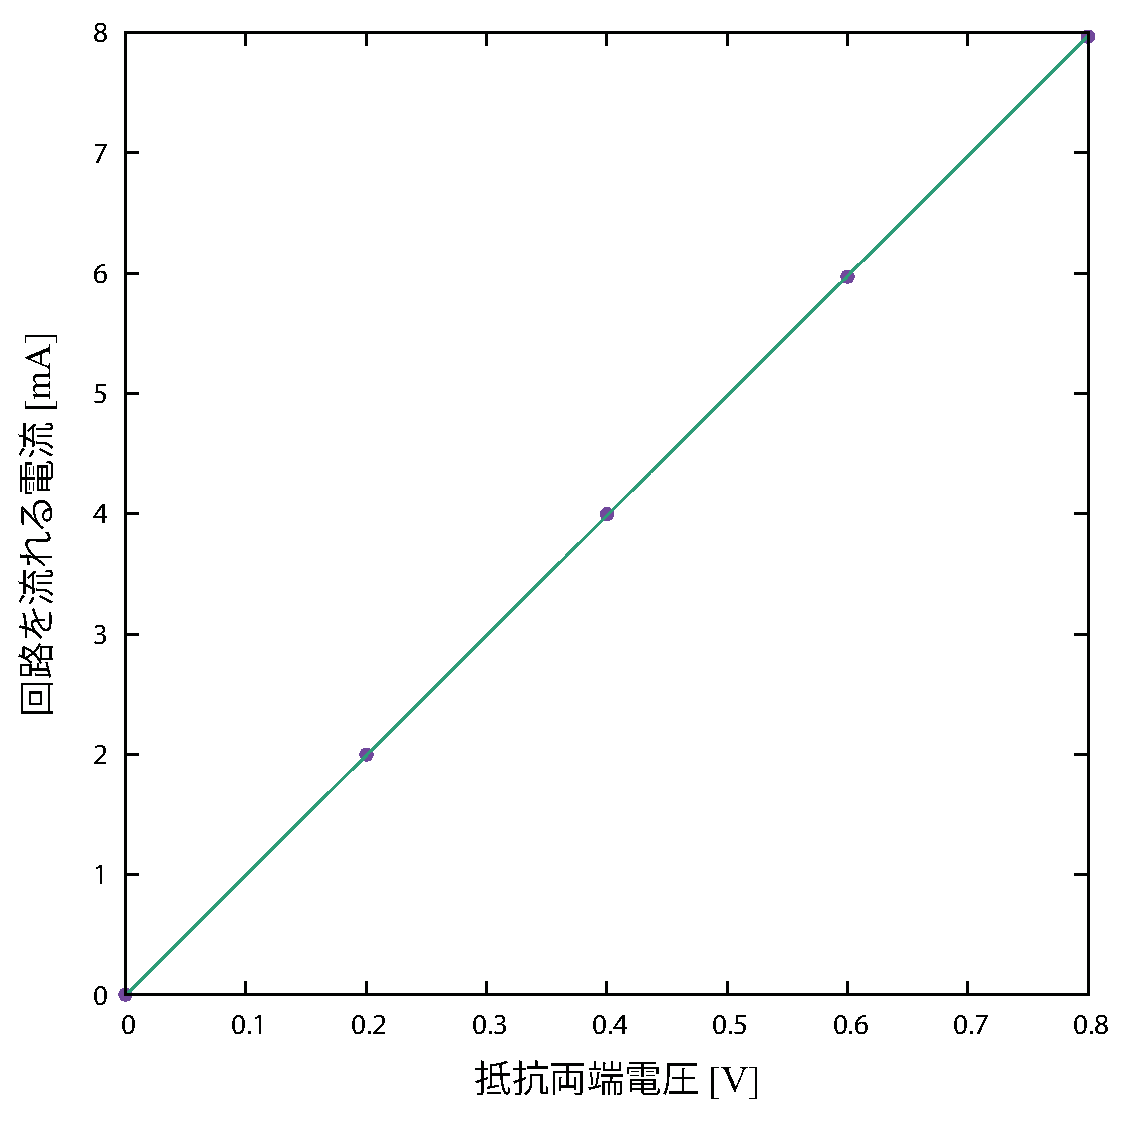
\includegraphics[scale=0.4]{ohm22.eps}
 \caption{何らかの法則を確認するために取得したデータをプロットした図}
 %\ecaption{Options of documentclass.}
 \label{ohm}
\end{center}
\end{figure}

実験結果のセクションでは,基本的に執筆者である皆さんがどのような思考過程を経て,
どのような数値データに基づいて結論に至ったのかが読者にわかるように提示することが
重要です.逆に言えば,それ以外の部分について(あるいは読者が容易に理解可能な
ことについて)逐一丁寧にこのセクションに記載する必要はありません(そういったものを
記載しなければならない場合は「付録」を上手に使うことを考慮してください).

典型的な事例として不確かさを計算する場合を挙げましょう.実験課題「光のスペクトル」では,
回折格子を用いて原子の光を分光してスペクトルの輝線を観察します.最初に波長がよくわかっている
ナトリウムのD$_1$線,D$_2$線を観測し,1次と2次の回折角をデータとして得て,回折格子の
格子定数 $N$ (単位長さあたり何本の溝が切ってあるか)を求めます.

格子定数の不確かさ $\Delta N$ は次の式,
%
\[
\frac{\Delta N}{N}=\sqrt{\left (\frac{\cos\theta}{\sin\theta}\right )^2+\left (\frac{\Delta \lambda}{\lambda}\right )^2}
\]

\noindent
によって不確かさの計算を行います.ここで $\theta$ は回折角,$\lambda$ および $\Delta \lambda$はナトリウムの
D$_1$,D$_2$線の波長で各々589.592nm,588.995nmです(物理量は1つの数値と1つの単位の
掛算で表されます.「589.592/nm」や「589.592[nm]」 という表し方は誤りです).この実験課題のレポートの
「実験結果」のセクションを書く要素としては次のことが考えられるでしょう.
\begin{itemize}
\setlength{\itemsep}{-3mm}
 \item 不確かさを計算する式(上式)
 \item 各不確かさ($\Delta\theta$,$\Delta\lambda$)にどのようなものを採用したのかを示す数値
 \item 具体的な計算(上式に数値を代入したもの)
 \item 不確かさの計算結果
\end{itemize}

最初の項目である不確かさをどのように計算するかの式は,もしこれがなく単に「テキストの式xxより」としてしまうと少し
雑な印象を与えるかもしれません.2つ目の項目は測定者のみが判断できることですから,
これを載せなければ以降の計算結果について読者な何も読み取ることはできません.3つ目の
項目はどうでしょうか?単純な四則演算を見せられても読者にとっては特に興味がないかもしれません.
もちろん,その計算に特別な意味があるなら載せなければなりません.最後の項目はもちろん
必要なことは分かると思います.

実験結果のセクションでは皆さんが測定で求めた数値について,その精度も含めて,また存在する場合には
文献値など比較可能な値と一緒に表でまとめてください.光のスペクトルの回折格子の格子定数に関する
例であれば,次のような表にしてまとめることになるでしょう.
%
\begin{table}[ht]
\begin{center}
\caption{NaのD$_1$,D$_2$線による回折格子の格子定数の測定結果}
\label{tab2}
\begin{tabular}{ccc}\hline
 &測定による格子定数 $N\pm \Delta N / \rm{mm}$ & 設計値 $N_0 / \rm{mm}$ \\ \hline
 一次D$_1$線 & 600.2$\pm$0.5 & \\
 一次D$_2$線 & 600.1$\pm$0.5 & \\
二次D$_1$線 & 600.1$\pm$0.2 & \\
二次D$_1$線 & 600.0$\pm$0.2 & \\ \hline
平均 & 600.1$\pm$0.2 & 600.0 \\ \hline
\end{tabular}
\end{center}
\end{table}


%%%%%%%%%%%%%%%%%%%%%%%%%%%%%%%%%%%%%%%%%%%%%%%%%%%%%%%%%%%%%%%%%%%%%%
\section{考察}

 考察を書くのは,特に初年次の実験では難しいものとなります.最初は次の2つのことを
目指して書くと良いでしょう.
%
\begin{itemize}
\setlength{\itemsep}{-3mm}
 \item 求めた数量に対する定量的な分析
 \item 実験課題に関係するトピックの調査結果(文献等を調べて書く,あるいは原理式を自分で解いてみるなど)
\end{itemize}

最も注意して欲しい点は,「考察」は「感想」とは違うということです.一例として(よく見かける考察の記述として),
 \vspace{2mm}
 
 「求めた結果は文献値とよく一致しており,この実験は成功したといえる.」 \\
 
 「求めた結果は文献値と大きく離れてしまっており,この実験は失敗だったと思う.\\
   次の実験からは失敗しないよう予習をきちんとやりたい.」

\vspace{2mm}
\noindent
というようなものがあります.これらは何故「考察」になっていないのでしょうか?
第一に「よく一致」や「大きく離れている」というのは主観的,感覚的な表現です.測定結果は
常にある精度の範囲で求まるものであり,測定値の精度は極端な言い方をすれば特定の測定装置を
選んだ時点で決定しています.求めた物理量はその精度の範囲でしかわかりませんから,
どのくらいの精度の範囲で比較するのか示さない議論は意味をなさないということになります.
第二に,そもそも測定によって決定する物理量は言うまでもなく一定の方法論にしたがって
得た測定値を用いて導いたもので,たまたま得られた偶然の値ではなく,それそのものは何らかの意味が
あるとみるべきものです(必然的に求まった数値ということです).自身の値を文献値または参考になる値と近い値だった,
あるいは遠く離れた値だったという基準で「良い」や「悪い」という評価をするものではありません.皆さんが
行った測定は何らかの原因,要因によって必然として得られるべき値が得られたと考えるものです(ただし,
再現性がないものについては再度確認を行う必要があります).

\newpage
\subsection{定量的な考察}
 以上を踏まえて定量的な考察の例を示すことにしましょう.考察をまとめる工程は単純で以下のような
方針です.
\begin{itemize}
\setlength{\itemsep}{-2mm}
 \item 求めた値と参考値,文献値との差が生じた原因がどの測定値にあるかアイディアを出す
 \item その測定がどの程度変化すれば差がなくなるのか計算する
 \item そのような差は,測定精度上起こりうるのか考え,起こりえない場合はそのアイディアは棄却する
\end{itemize}
 
 具体的な例として再び「液体の比熱」を例にとってみます.ある学生が加熱の実験を行い,その
 実験レポートの「実験結果」のセクションの最後に次の表が掲げられていたとしましょう.
%
\begin{table}[ht]
\begin{center}
\caption{加熱法による水の比熱の実験結果}
\label{tab3}
\begin{tabular}{ccc}\hline
 & 測定値 & 文献値 \\ \hline
$C/\rm{J \cdot g^{-1} \cdot K^{-1}} $ &  3.1$\pm$ 0.1 & 4.217 \\ \hline
\end{tabular}
\end{center}
\end{table}

加熱法による比熱は式(\ref{eq4})より,$\Delta T/\Delta t=a$ とすれば,
\[
C=\frac{1}{M}\left (\frac{Ri^2}{a}-mc\right )
\]
から計算します.この学生の測定では水の質量 $M=174.54 \rm{g}$,加熱用コイルの抵抗値 $R=4.331 \rm{\Omega}$,
電流 $i=1.66 \rm{A}$,熱量計の質量 $m=63.93 \rm{g}$file:///C:/Users/dummy/Documents/実験/基礎科学実験A/hcap2.eps
 の諸量を使っており,データをグラフにプロットした
図から傾きを $a=2.145\times 10^{-2}\, \tempC\rm{\cdot s^{-1}}$ として比熱を計算しています.

文献値との差は26\%ほど乖離しています.この差はどこからくるものでしょうか?計算に用いた諸量の
うち,抵抗値,電流値,
熱量計の質量,熱量計(銅)の比熱は測り間違いは考えにくく,また測定を繰り返したとしても
それほどの大きな違いは出ないように思えます.そこで文献値との差が生じた原因は,
水の質量とグラフから読み取った直線の傾きが影響していると考えるのがよさそうです(アイディアの提起).

では,仮に水の質量の変化あるいは測り間違いが今回の実験結果に影響を与えたとし,
他の測定値は適正に得られたと仮定すると文献値の比熱を与える値はどのようなものだったのかを
計算してみます.これは
\[
M=126.10 \rm{g}
\]

\noindent
でなければなりません.1/100 g まで測定できる電子天秤を使っている中で,水の質量が
40 gも変化しなければならないというのは全く現実的ではないでしょうから,この
仮定は捨て去る必要がありそうです.

グラフの傾きはどうでしょうか?同様に計算をすると文献値に近い比熱を与える傾きは,
\[
a=1.57\times 10^{-1}\,\tempC  \rm{/s}
\]

\noindent
となります.
%
\begin{figure}[ht]
\begin{center}
 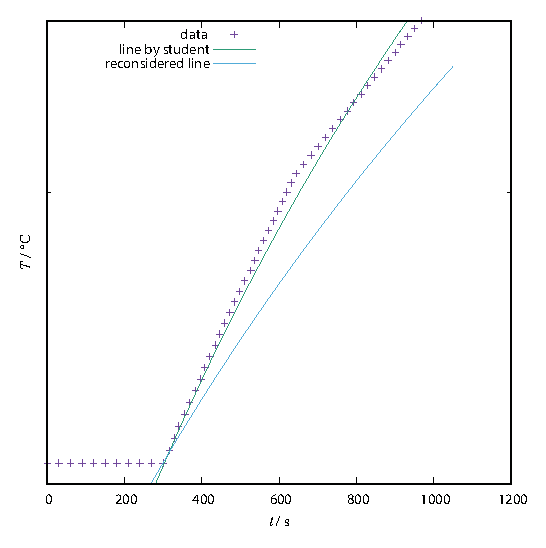
\includegraphics[scale=0.8]{hcap.eps}
 \caption{水の加熱データのプロット.下側の線が文献値に近い値を与える傾きの直線.}
 %\ecaption{Options of documentclass.}
 \label{hcap-plt}
\end{center}
\end{figure}

以下にこの学生が決定した傾きと文献値に近い比熱を与える傾きの直線をデータとともに
示しましょう.
図\ref{hcap-plt}を見ればわかる通り,この加熱データは文献値に近い比熱を与える
直線の傾きに対して全領域で上側に移動していることがわかります.つまり,測定データは
本来の温度上昇よりも大きな値を示していたということになりそうです.こういった差が
何故生じたのかについては,例えば液温を測る温度計の測温部がコイルの近傍に
あったため,というアイディアはどうでしょうか?それとも他に何かアイディアはあるでしょうか?

%\vspace{3mm}
\newpage
残念ながら,この実験のデータは実際に得られるものよりも少し異なる結果になっている
可能性があるようです.そのようなことが発生した原因として考えられるものは幾つか
挙げられますが残念ながら取得したデータから数値的に検証するのは困難です.
しかし,もしも次にデータをとる機会があるならば,それを検証するためにどのような
測定を行えばよいのか提案することは良いことです.例えば測温部とヒータの位置関係を
故意にずらし,その間の距離と温度データを幾つか取得するというのはどうでしょうか?
今回の仮説を立証するために必要な情報を得られないでしょうか?

このように,考察ではアイディアを上げたら具体的に数値を計算しながら(これが定量的にという
意味です),検討を加えていくことが必要です.もちろん時として得られたデータからだけでは
解決しない場合もあります.そのようなときは次の機会にどういった測定を行えばよいのかを
提案するようにしましょう.

\subsection{文献を調べて調査する・原理式を詳細に調べてみる}
実験課題に関連することについて文献を調べたことを考察に書く,あるいは原理式で使われている数式を
自分で計算してみるというのも考察に書く内容としてはふさわしいことです.初年次の実験では
多くは皆さんがまだ習っていないトピックを取り扱います.例えば重力加速度では式(\ref{eq1})を
原理式としていますが,この式はそれほど自明なものではなく,考察に(全て理解したうえでなくとも)
どのように導かれるのか,各項の物理的な意味を解説するのは意味があることです.また粘性率では
原理式としてポアズイユの法則を用いています.この法則は粘性を持った流体の流量が圧力差と
毛細管の半径の4乗に比例し,粘度に逆比例するというものです.テキストでは比例係数を
含めて書かれていますが,流量 $V$ と圧力差 $\Delta P$,毛細管の半径 $a$,流体の
粘度を $\eta$ としたとき,
\[
V\propto \frac{a^4\Delta P}{\eta}
\]

\noindent
となることを追跡する(自分で式を追って計算してみる)ことはそれほど難しい問題ではありません.

\vspace{3mm}
以上で考察にどのようなことを書いていけばよいか簡単に紹介をしました.考察を書き上げることは
なかなか難しいことであって,半期の授業の中で完全に身につくものではありません.より良いものを
書くことができるよう練習を続けてください.

%%%%%%%%%%%%%%%%%%%%%%%%%%%%%%%%%%%%%%%%%%%%%%%%%%%%%%%%%%%%%%%%%%%%%%
\section{その他}
このファイルでは画像はeps形式のファイルを使っていますが,png等の画像を直接
貼り付けることも可能です.次のようにします.
\begin{verbatim}
\begin{figure}[ht]
\begin{center}
 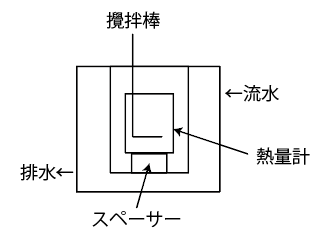
\includegraphics[scale=0.6]{aparatus2.png}
 \caption{実験装置の概略図}
 \label{apara}
\end{center}
\end{figure}
\end{verbatim}

レポートでは考察の後に「まとめ」を入れることもあります.「まとめ」では行った実験から
どのようなことが判明したのか(自分が理解したことではなく,実験結果から物理現象に
対する知見としてどのような性質があることが分かったのか)を書きます.しかし,すでに
触れたとおり,基礎科学実験Aを受講する皆さんは場合によっては未知の学習項目に
ついて実験をする場合も多くあり,そのような中で「まとめ」を書くのはなかなか難しい問題ですから
省略しても構いません.

\vspace{3mm}
考察(あるいはまとめ)まで書いたら「参考文献」のセクションを書きます.参考文献は
セクション番号を入れない場合が多いようです.「参考文献」とは書かずに横線を引くような
ケースもあります.いずれの場合も自身がレポートを作成するにあたって参照した他者の著作物は,
このセクションの中に文献番号を付けて列挙していきます.その際,
本文中で文献を引用したところに文献番号を付けます.文献の列挙の仕方はoo方式のような
ものは存在します.大まかな習慣はありますが,詳細な部分では研究分野のコミュニティーごとに
違いはあるようです.文献の列挙の一例は以下のとおりです.\TeX の場合はbibliography環境を
使えば書式を気にせずに書くことができます.

\vspace{2mm}
[1] 著者名/編者名,書名, 発行所,発行都市,発行年. 

[2] 著者名,表題,雑誌名,巻号,ページ,発行年.

[3] 著者名/組織名,URL,最終アクセス日.

$\vdots$

\vspace{3mm}
レポートを書くにあたってただの1つも参考文献がないのはおよそ考え難いことです(ここ100年の間では
唯一,A. アインシュタイン博士が特殊相対性理論の論文を公表した際に一切の参考文献が
なかったと言われています.しかし,彼の天才性をもってしてなお批判があったようです).逆に言えば
参考文献がないようなレポートは内容の如何に関わらず水準に達していないといって良いでしょう.
多くの場合テキストは参考文献にカウントされません.積極的に文献を調べてレポートを作成して
ください.なお,最近ではWEBを参照する場合が多くなってきましたが,WEBの情報は誰もが
簡単に発信できるものですから,信頼性には十分留意する必要があります(1つのソースだけでなk
複数のソースで確認するなど).以下は参考文献の書き方の例です(\TeX の場合は bibliography環境を
使えば標準的な参考文献.

%%%%%%%%%%%%%%%%%%%%%%%%%%%%%%%%%%%%%%%%%%%%%%%%%%%%%%%%%%%%%%%%%%%%%%
\begin{thebibliography}{99}
\bibitem{Eijkhout}
M.Kobayashi and T.Maskawa, ``CP-Violation in the Renormalizable Theory
	of Weak Interaction'', Prog.Theor. Phys., Vol.49 No.2, pp.652-657, 1973.

\bibitem{tex}
D.E. クヌース,改訂新版 \TeX\ ブック,アスキー出版局,東京,1992. 

\bibitem{Bech}
S. von Bechtolsheim, \TeX\ in Practice, Springer-Verlag, New York, 1993. 

\bibitem{hujita}
藤田眞作,化学者・生化学者のための\LaTeX---パソコンによる論文作成の手引,
東京化学同人,東京,1993. 

\bibitem{Ase}
阿瀬はる美,``てくてく\TeX{}'',
アスキー出版局,東京,1994. 

\bibitem{Walsh}
N. Walsh, Making \TeX\ Work, O'Reilly \& Associates, Sebastopol, 1994. 

\bibitem{Salomon}
D. Salomon, The Advanced \TeX\ book, Springer-Verlag, New York, 1995.

\bibitem{hujita4}
川上三郎,川口四郎,``紫外域半導体レーザ'',1995 電気通信大学技術発表会,
	no.123,pp.20-21,Mar. 1995.

%\bibitem{last}
%T.Hayashi, Y.Koide, M.Matsuda, M.Tanimoto, ``Neutron Electric Dipole
%	Moment in Two Higgs Doublet Model'',Prog.Theor. Phys., Vol.91 No.5, pp.915-926, 1994.
\end{thebibliography}

%%%%%%%%%%%%%%%%%%%%%%%%%%%%%%%%%%%%%%%%%%%%%%%%%%%%%%%%%%%%%%%%%%%%%%
\appendix
\setcounter{figure}{0}
\setcounter{table}{0}
\numberwithin{equation}{section}
\renewcommand{\thetable}{\Alph{section}\arabic{table}}
\renewcommand{\thefigure}{\Alph{section}\arabic{figure}}
%\def\thesection{付録\Alph{section}}
\makeatletter 
\newcommand{\section@cntformat}{付録 \thesection:\ }
\makeatother
%%%%%%%%%%%%%%%%%%%%%%%%%%%%%%%%%%%%%%%%%%%%%%%%%%%%%%%%%%%%%%%%%%%%%%

\section{付録の書き方}
 本文に掲載すると煩雑になるような場合で,しかしもう少し詳細に触れなければならないような
ものについては「付録」を利用して掲載する方法もあります.付録ではセクション番号を
大文字のアルファベットにしたりする場合もあります.またこれに応じて式番号も A-1, A-2のように
本文とは違うように書くようにします(図表のキャプションも同様に変えます).

数式番号は上の\%で囲まれた部分で設定をしていますので,皆さんが特に何かを設定する
必要はありません.
\begin{equation}
 E=mc^2
 \label{eq-ae}
 \end{equation}

このように表示されます.またこのように\verb|\ref{<label>}| としてレファレンスすれば(\ref{eq-ae})のように
正しく参照されます.

%
\begin{table}[ht]
\begin{center}
\caption{加熱法による水の比熱の実験結果}
\label{tabA1}
\begin{tabular}{ccc}\hline
 & 測定値 & 文献値 \\ \hline
$C/\rm{J \cdot g^{-1} \cdot K^{-1}} $ &  3.1$\pm$ 0.1 & 4.217 \\ \hline
\end{tabular}
\end{center}
\end{table}

付録には必ずしも掲載するのが必要でないデータの表や,計算の詳細を載せるのに
使うとよいでしょう.ただし,データを全て付録にしてしまうことには慎重であるべきです.
既に記したとおり,本文では皆さんがどのように考え,そのような方法論で結論を
得たのかについて,読者が疑問に思わないように必要なデータ,グラフを掲載することを
忘れないでください.

%%%%%%%%%%%%%%%%%%%%%%%%%%%%%%%%%%%%%%%%%%%%%%%%%%%%%%%%%%%%%%%%%%%%%%
\end{document}

\begin{figure}[ht]
\begin{center}
 \includegraphics[scale=0.5]{ファイル名}
 \caption{タイトル}
 %\ecaption{Options of documentclass.}
 \label{apara}
\end{center}
\end{figure}

\begin{table}[ht]
\begin{center}
\caption{タイトル}
\label{tab1}
\begin{tabular}{ll}\hline
col1 & col2 \\ \hline
val1 & val2 \\
val3 & val4 \\ \hline
\end{tabular}%
\end{center}
\end{table}
